\documentclass[12pt]{article}
\usepackage{fancyhdr}
\usepackage{color}
\usepackage{multicol}
\usepackage{enumitem}
\usepackage{graphicx}
\usepackage{sectsty}
\usepackage{amsmath}
\usepackage{amssymb}
\usepackage{hyperref}
\usepackage{array}
\newcommand{\sectionbreak}{\clearpage}

\usepackage{tikz}
	\usetikzlibrary{arrows,shapes,trees}


\allsectionsfont{\centering}

\usepackage{draftwatermark}
	\SetWatermarkText{\copyright wolf-math.com}
	\SetWatermarkScale{4}
	\SetWatermarkLightness{1}

\usepackage[margin=1in, headsep=0pt]{geometry}
\setlength{\parindent}{0cm}
\pagestyle{empty}

\begin{document}

Mr. Wolf  \\ wolf-math.com

\section*{Trig Pre-Requisites}

\subsection*{Goals}

\textbf{SWBAT} calculate and apply the Pythagorean Theorem.\\

\textbf{SWBAT} calculate and apply the distance formula.\\

\textbf{SWBAT} graph circles using $x^2+y^2=r^2$\\

\subsection*{Standards}

\textbf{Expressing Geometric Properties with Equations \hfill	G-GPE}\\

Translate between the geometric description and the equation for a
conic section\\

1.Derive the equation of a circle of given center and radius using the
Pythagorean Theorem; complete the square to find the center and
radius of a circle given by an equation.\\

Use coordinates to prove simple geometric theorems algebraically\\

7.	 Use coordinates to compute perimeters of polygons and areas of
triangles and rectangles, e.g., using the distance formula. \\

\textbf{Geometry \hfill 8.G}\\

Understand and apply the Pythagorean Theorem.\\

6.	 Explain a proof of the Pythagorean Theorem and its converse.\\
7.	 Apply the Pythagorean Theorem to determine unknown side lengths
in right triangles in real-world and mathematical problems in two and
three dimensions.\\
8.	 Apply the Pythagorean Theorem to find the distance between two
points in a coordinate system.\\

\subsection*{Connections}

\textbf{Now} we are learning the equation of a circle, the Pythagorean Theorem and the distance formula, all of which are prerequisites to trigonometry.\\

\textbf{Later} we are going to learn basic trig ratios and how to solve right triangles with those ratios.\\

\let\stdsection\section
\renewcommand\section{\newpage\stdsection}

\section*{The Pythagorean Theorem}

$$a^2+b^2=c^2$$

Given any right triangle, if the lengths of the legs (the shorter sides) are known, but the hypotenuse (the longest side) is unknown, the length of the hypotenuse can be figured out with the Pythagorean Theorem, $a^2+b^2=c^2$, where $a$ and $b$ are the legs, and $c$ is the hypotenuse.\\

\textbf{Example:} 

\pagebreak

\section*{The Distance Formula}

An application of the \textit{Pythagorean Theorem} is the \textbf{Distance Formula}. With it the distance between two points on a graph can be calculated.\\

$$d=\sqrt{(x_1-x_2)^{2}+(y_1-y_2)^{2}}$$

\textbf{Example:} 1) Let point a be $(1,1)$, and point b be $(4,5)$. Find the distance between them.\\

\begin{center}
%\includegraphics[scale=.5]{graph1.jpg}\\
\end{center}

With the distance formula the distance can be calculated without graphing.\\

\textbf{Example 2:} Find the distance between $(2,3)$ and $(4,5)$.\\

\vspace{1cm}

\textbf{Example 2:} $(0,0)$ to $(5,5)$.\\

\vspace{1cm}

\textbf{You Try:}

\begin{enumerate}
	
	\item $(-4,10)$ and $(7,-6)$\\

	\item $(10,2)$ and $(12, 17)$\\

	\item $(-1,-5)$ and $(4,-6)$\\

\end{enumerate}


\section*{Equation of a Circle}

\subsection*{Graphing Circles}

A circle whose center is about the origin can be graphed with the equation $$r^2=x^2+y^2$$ where $r$ is the radius, $x$ is the $x$ coordinate, and $y$ is the $y$ coordinate. \\

\textbf{Example 1:} $x^2+y^2=1$

\begin{center}
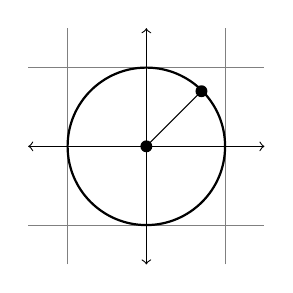
\begin{tikzpicture}[scale=1.]

	\draw[help lines] (-1.5,-1.5) grid (1.5,1.5);
	\draw[style=thick] (0,0) circle (1);
	\draw[<->] (-1.5,0) -- (1.5,0);
	\draw[<->] (0,1.5) -- (0,-1.5);
	\draw (0,0) -- (.7,.7);
	\fill[black] (.7,.7) circle (.5ex);
	\fill[black] (0,0) circle (.5ex);

\end{tikzpicture}
\end{center}

\textbf{Example 2:} $x^2+y^2=4$ -- what's the radius?

\begin{center}
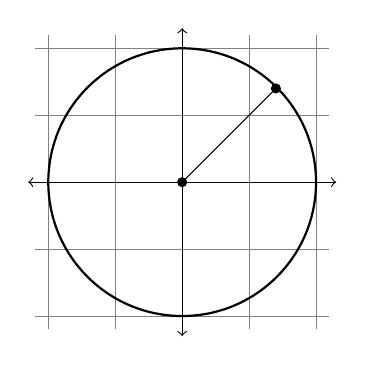
\begin{tikzpicture}[scale=.85]

	\draw[help lines] (-2.2,-2.2) grid (2.2,2.2);
	\draw[style=thick] (0,0) circle (2);
	\draw[<->] (-2.3,0) -- (2.3,0);
	\draw[<->] (0,2.3) -- (0,-2.3);
	\draw (0,0) -- (1.414,1.414);
	\fill[black] (1.4,1.4) circle (.5ex);
	\fill[black] (0,0) circle (.5ex);

\end{tikzpicture}
\end{center}




The circle can be moved around. In the following equation the center would be at the point $(h,k)$. Notice that there are minus signs in the parentheses.

$$r^2=(x-h)^2+(y-k)^2$$

\textbf{Example 3:} $9=(x-2)^2+(y+3)^2$ 

\begin{center}
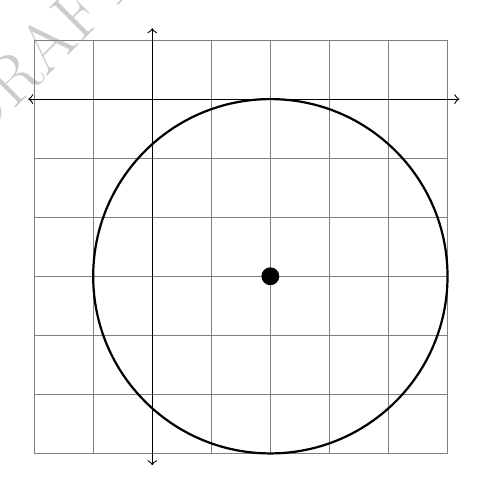
\begin{tikzpicture}[scale=.75]

	\draw[help lines] (-2,-6) grid (5,1);
	\draw[<->] (-2.1,0) -- (5.2,0);
	\draw[<->] (0,1.2) -- (0, -6.2);
	\draw[style=thick] (2,-3) circle (3);
	\fill[black] (2,-3) circle (1ex);

\end{tikzpicture}
\end{center}

\pagebreak

\subsection*{Writing Equations of Circles}

$$r^2=(x-h)^2+(y-k)^2$$

We can write the equation of any circle given certain information.\\

\textbf{Example 4:} Center at $(-1,4)$, radius $=3$

\vspace{1in}

\textbf{You Try:} Center at $(2,4)$, radius $=6$

\vspace{1in}

\hrulefill

\textbf{Example 5:} Center at $(-5,-2)$ point on circle $(1,1)$\\
\textbf{Hint:} The distance between them is the radius.\\

\vspace{1in}

\textbf{You Try:} Center at $(-5,-4)$ point on circle $(-4,-2)$

\vspace{1in}


\hrulefill

\textbf{Example 6:} What is the equation of this graph?

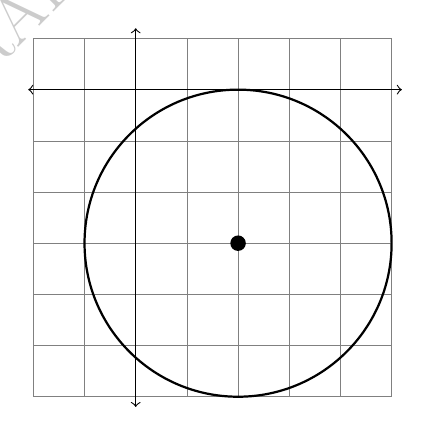
\begin{tikzpicture}[scale=.65]

	\draw[help lines] (-2,-6) grid (5,1);
	\draw[<->] (-2.1,0) -- (5.2,0);
	\draw[<->] (0,1.2) -- (0, -6.2);
	\draw[style=thick] (2,-3) circle (3);
	\fill[black] (2,-3) circle (1ex);

\end{tikzpicture}

\section*{Review So Far...}

Mr. Wolf \hfill \textbf{NAME:\underline{\hspace{2in}}}\\
Pre-Calculus \hfill \textbf{Date: \underline{\hspace{1in}}}\\

\subsection*{Pythagorean Theorem}

Given the triangle diagram below, determine the unknown distance.

$$a^2+b^2=c^2 \hspace{1in} c=\sqrt{a^2+b^2}$$

\begin{center}
	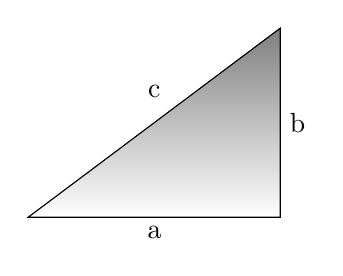
\begin{tikzpicture}[scale=.8]
	
		\path[draw, shade] (0,0) -- 
			(4,0) node[pos=.5,below] {a} -- 
			(4,3)node[pos=.5,right] {b} --cycle;
			
			\node (c) at (2,2) {c};
	
	\end{tikzpicture}
\end{center}

\begin{enumerate}
	\item $a=6$, \hspace{1cm} $b=6$,\hspace{1cm} $c=$\underline{\hspace{1in}}\\
	
	\item $a=$\underline{\hspace{1in}}, \hspace{1cm}$b=12$,\hspace{1cm} $c=15$\\
	
	\item $a=8$, \hspace{1cm}$b=6$, \hspace{1cm}$c=$\underline{\hspace{1in}}\\
	
	\item $a=5$, \hspace{1cm}$b=$\underline{\hspace{1in}}, \hspace{1cm}$c=5\sqrt{2}$\\
	
	\item $a=10$,\hspace{1cm} $b=\sqrt{21}$,\hspace{1cm} $c=$\underline{\hspace{1in}}
\end{enumerate}


\hrulefill

\subsection*{The Distance Formula}

$$d=\sqrt{(x_{1}-x_{2})^{2}+(y_{1}-y_{2})^{2}}$$

Find the distance between the two points.\\

\begin{enumerate}[resume]
\begin{multicols}{2}

	\item $(0,0),(12,5)$\\
	
	\item $(-3,-5),(5,10)$\\
	
	\item $(-10,-10),(10,11)$\\
	
	\item $(-5,2), (19,-5)$\\
	
	\item $(4,-2),(-1,8)$\\

\end{multicols}
\end{enumerate}

\pagebreak

\subsection*{Equation of a Circle}

$$r^2=x^2+y^2$$

$$r^2=(x-h)^2+(y-k)^2$$

Write the equation of a circle with the following criteria\\

\begin{enumerate}[resume]

	\item $r=4$, center at the origin\\
	
	\item $r=9$, center at $(4,9)$\\
	
	\item $r=1$, center at $(-1,-1)$\\
	
	\item $r=\sqrt{2}$, center at $(-3,7)$\\
	
	\item $r=\sqrt{5}$, center at $(5,-1)$\\
	
	\item center at origin, passes through the point $(9,40)$\\
	
	
\end{enumerate}

\hrulefill

Sketch the following equations.\\

\begin{enumerate}[resume]
\begin{multicols}{2}

	\item $x^2+y^2=4$\\
	
%	\includegraphics[scale=.5]{graph1.jpg}
	
	\item $(x-1)^2+(y+3)^2=9$\\
	
%	\includegraphics[scale=.5]{graph1.jpg}

\end{multicols}
\end{enumerate}

\section*{Review}

Mr. Wolf \hfill \textbf{NAME:\underline{\hspace{2in}}}\\
Pre-Calculus \hfill \textbf{Date: \underline{\hspace{1in}}}\\

\subsection*{Pythagorean Theorem}

Given the triangle diagram below, determine the unknown distance. (2 points each)

$$a^2+b^2=c^2 \hspace{1in} c=\sqrt{a^2+b^2} \hspace{1in} a=\sqrt{c^2-b^2}$$

\begin{center}
	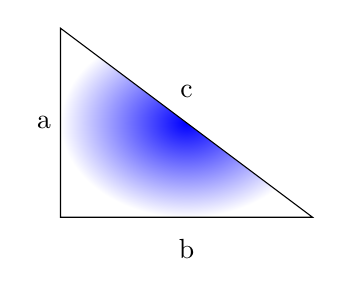
\begin{tikzpicture}[scale=.8]
	
		\path[draw,  inner color=blue ] (0,0)-- 
			(0,3) node[pos=.5,left] {a} -- 
			(4,0) --cycle;
			
			\node (c) at (2,2) {c};
			\node (b) at (2,-.5) {b};
			
	
	\end{tikzpicture}
\end{center}

\begin{enumerate}
	\item $a=21$, \hspace{1in} $b=20$,\hspace{1in} $c=$\underline{\hspace{1in}}\\
	
	\item $a=$\underline{\hspace{1in}}, \hspace{.5cm} $b=40$,\hspace{1in} $c=41$\\
	
	\item $a=15$, \hspace{1in}$b=8$, \hspace{1in}$c=$\underline{\hspace{1in}}\\
	
	\item $a=1$, \hspace{1in}$b=$\underline{\hspace{1in}},\hspace{.5cm} $c=\sqrt{2}$\\
	
	\item $a=1$,\hspace{1in} $b=\sqrt{2}$,\hspace{1in} $c=$\underline{\hspace{1in}}
\end{enumerate}


\hrulefill

\subsection*{The Distance Formula}

$$d=\sqrt{(x_{1}-x_{2})^{2}+(y_{1}-y_{2})^{2}}$$

Find the distance between the two points. (3 points each)\\

\begin{enumerate}[resume]
\begin{multicols}{2}

	
	\item $(-5,0),(3,15)$\\
	
	\item $(-13,-7),(7,14)$\\
	
	\item $(-5,2), (19,-5)$\\
	
	\item $(5,-2),(0,8)$\\

\end{multicols}
\end{enumerate}

\pagebreak

\subsection*{Equation of a Circle}

$$r^2=x^2+y^2$$

$$r^2=(x-h)^2+(y-k)^2$$

Write the equation of a circle with the following criteria. (2 points each)\\

\begin{enumerate}[resume]

	\item $r=3$, center at the origin\\
	
	\item $r=5$, center at $(3,-5)$\\
	
	\item $r=7$, center at $(-2,-9)$\\
	
	\item $r=\sqrt{5}$, center at $(-2,4)$\\
	
	\item $r=\sqrt{8}$, center at $(6,-2)$\\
	
	\item center at $(1,1)$, passes through the point $(15,12)$\\
	
	
\end{enumerate}

\hrulefill

Sketch the following equations. (3 points each)\\

\begin{enumerate}[resume]
\begin{multicols}{2}

	\item $x^2+y^2=16$\\
	
%	\includegraphics[scale=.5]{graph1.jpg}
	
	\item $(x+2)^2+(y-3)^2=4$\\
	
%	\includegraphics[scale=.5]{graph1.jpg}

\end{multicols}
\end{enumerate}


\section*{Quiz.}

Mr. Wolf \hfill \textbf{NAME:\underline{\hspace{2in}}}\\
Pre-Calculus \hfill \textbf{Date: \underline{\hspace{1in}}}\\

\subsection*{Pythagorean Theorem}

Given the triangle diagram below, determine the unknown distance. (2 points each)

$$a^2+b^2=c^2 \hspace{1in} c=\sqrt{a^2+b^2} \hspace{1in} a=\sqrt{c^2-b^2} \hspace{1in} b=\sqrt{c^2-a^2}$$

\begin{center}
	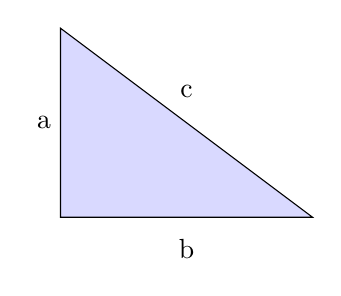
\begin{tikzpicture}[scale=.8]
	
		\path[draw, fill=blue!15 ] (0,0)-- 
			(0,3) node[pos=.5,left] {a} -- 
			(4,0) --cycle;
			
			\node (c) at (2,2) {c};
			\node (b) at (2,-.5) {b};
			
	
	\end{tikzpicture}
\end{center}

\begin{enumerate}
	\item $a=10$, \hspace{1in} $b=24$,\hspace{1in} $c=$\underline{\hspace{1in}}\\
	
	\item $a=$\underline{\hspace{1in}}, \hspace{.5cm} $b=80$,\hspace{1in} $c=82$\\
	
	\item $a=6$, \hspace{1in}$b=8$, \hspace{1in}$c=$\underline{\hspace{1in}}\\
	
	\item $a=1$, \hspace{1in}$b=$\underline{\hspace{1in}},\hspace{.5cm} $c=\sqrt{3}$\\
	
	\item $a=1$,\hspace{1in} $b=1$,\hspace{1in} $c=$\underline{\hspace{1in}}
\end{enumerate}


\hrulefill

\subsection*{The Distance Formula}

$$d=\sqrt{(x_{1}-x_{2})^{2}+(y_{1}-y_{2})^{2}}$$

Find the distance between the two points. (3 points each)\\

\begin{enumerate}[resume]
\begin{multicols}{2}

	
	\item $(-5,0),(-2,-4)$\\
	
	\item $(-13,-20),(-4,20)$\\
	
	\item $(-5,2), (0,14)$\\
	
	\item $(5,-2),(-3,10)$\\

\end{multicols}
\end{enumerate}

\pagebreak

\subsection*{Equation of a Circle}

$$r^2=x^2+y^2$$

$$r^2=(x-h)^2+(y-k)^2$$

Write the equation of a circle with the following criteria. (2 points each)\\

\begin{enumerate}[resume]

	\item $r=4$, center at the origin\\
	
	\item $r=6$, center at $(-3,-4)$\\
	
	\item $r=2$, center at $(0,7)$\\
	
	\item $r=\sqrt{3}$, center at $(9,7)$\\
	
	\item $r=\sqrt{7}$, center at $(6,0)$\\
	
	\item center at $(0,0)$, passes through the point $(33,56)$\\
	
	
\end{enumerate}

\hrulefill

Sketch the following equations. (3 points each)\\

\begin{enumerate}[resume]
\begin{multicols}{2}

	\item $x^2+y^2=25$\\
	
%	\includegraphics[scale=.75]{graph1.jpg}
	
	\item $(x-1)^2+(y+1)^2=16$\\
	
%	\includegraphics[scale=.75]{graph1.jpg}

\end{multicols}
\end{enumerate}

\section*{Quiz:}

Mr. Wolf \hfill \textbf{NAME:\underline{\hspace{2in}}}\\
Pre-Calculus \hfill \textbf{Date: \underline{\hspace{1in}}}\\

\subsection*{Pythagorean Theorem}

Given the triangle diagram below, determine the unknown distance. (2 points each)

$$a^2+b^2=c^2 \hspace{1in} c=\sqrt{a^2+b^2} \hspace{1in} a=\sqrt{c^2-b^2} \hspace{1in} b=\sqrt{c^2-a^2}$$

\begin{center}
	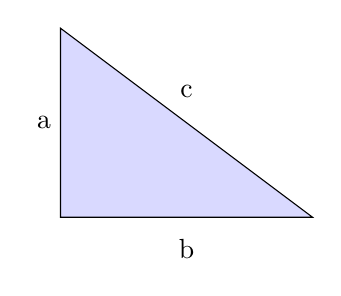
\begin{tikzpicture}[scale=.8]
	
		\path[draw, fill=blue!15 ] (0,0)-- 
			(0,3) node[pos=.5,left] {a} -- 
			(4,0) --cycle;
			
			\node (c) at (2,2) {c};
			\node (b) at (2,-.5) {b};
			
	
	\end{tikzpicture}
\end{center}

\begin{enumerate}
	\item $a=5$, \hspace{1in} $b=12$,\hspace{1in} $c=$\underline{\hspace{1in}}\\
	
	\item $a=$\underline{\hspace{1in}}, \hspace{.5cm} $b=40$,\hspace{1in} $c=41$\\
	
	\item $a=9$, \hspace{1in}$b=12$, \hspace{1in}$c=$\underline{\hspace{1in}}\\
	
	\item $a=2$, \hspace{1in}$b=$\underline{\hspace{1in}},\hspace{.5cm} $c=3$\\
	
	\item $a=2$,\hspace{1in} $b=2$,\hspace{1in} $c=$\underline{\hspace{1in}}
\end{enumerate}


\hrulefill

\subsection*{The Distance Formula}

$$d=\sqrt{(x_{1}-x_{2})^{2}+(y_{1}-y_{2})^{2}}$$

Find the distance between the two points. (3 points each)\\

\begin{enumerate}[resume]
\begin{multicols}{2}

	\item $(-15,-10),(-6,30)$\\
	
	\item $(7,-2),(-1,10)$\\
	
	\item $(0,10),(3,6)$\\
	
	\item $(3,0), (8,12)$\\

\end{multicols}
\end{enumerate}

\pagebreak

\subsection*{Equation of a Circle}

$$r^2=x^2+y^2$$

$$r^2=(x-h)^2+(y-k)^2$$

Write the equation of a circle with the following criteria. (2 points each)\\

\begin{enumerate}[resume]

	\item $r=1$, center at the origin\\
	
	\item $r=2$, center at $(3,-4)$\\
	
	\item $r=3$, center at $(-2,12)$\\
	
	\item $r=\sqrt{5}$, center at $(-10,-10)$\\
	
	\item $r=\sqrt{11}$, center at $(-1,2)$\\
	
	\item center at $(-10,-10)$, passes through the point $(23,46)$\\
	
	
\end{enumerate}

\hrulefill

Sketch the following equations. (3 points each)\\

\begin{enumerate}[resume]
\begin{multicols}{2}

	\item $x^2+y^2=25$\\
	
%	\includegraphics[scale=.75]{graph1.jpg}
	
	\item $(x-1)^2+(y+1)^2=16$\\
	
%	\includegraphics[scale=.75]{graph1.jpg}

\end{multicols}
\end{enumerate}

\section*{Quiz.:}

Mr. Wolf \hfill \textbf{NAME:\underline{\hspace{2in}}}\\
Pre-Calculus \hfill \textbf{Date: \underline{\hspace{1in}}}\\

\subsection*{Pythagorean Theorem}

Given the triangle diagram below, determine the unknown distance. (2 points each)

$$a^2+b^2=c^2 \hspace{1in} c=\sqrt{a^2+b^2} \hspace{1in} a=\sqrt{c^2-b^2} \hspace{1in} b=\sqrt{c^2-a^2}$$

\begin{center}
	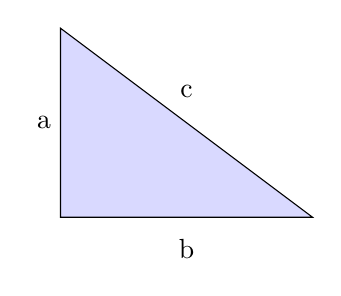
\begin{tikzpicture}[scale=.8]
	
		\path[draw, fill=blue!15 ] (0,0)-- 
			(0,3) node[pos=.5,left] {a} -- 
			(4,0) --cycle;
			
			\node (c) at (2,2) {c};
			\node (b) at (2,-.5) {b};
			
	
	\end{tikzpicture}
\end{center}

\begin{enumerate}

	\item $a=3$,\hspace{1in} $b=3$,\hspace{1in} $c=$\underline{\hspace{1in}}\\

	\item $a=70$, \hspace{1in} $b=24$,\hspace{1in} $c=$\underline{\hspace{1in}}\\
	
	\item $a=2$, \hspace{1in}$b=$\underline{\hspace{1in}},\hspace{.5cm} $c=3$\\
	
	\item $a=15$, \hspace{1in}$b=20$, \hspace{1in}$c=$\underline{\hspace{1in}}\\	
	
	\item $a=$\underline{\hspace{1in}}, \hspace{.5cm} $b=80$,\hspace{1in} $c=89$\\
\end{enumerate}


\hrulefill

\subsection*{The Distance Formula}

$$d=\sqrt{(x_{1}-x_{2})^{2}+(y_{1}-y_{2})^{2}}$$

Find the distance between the two points. (3 points each)\\

\begin{enumerate}[resume]
\begin{multicols}{2}

	
	\item $(0,0), (5,12)$\\
		
	\item $(-6,1),(-3,-3)$\\
	
	\item $(-10,-20),(-1,20)$\\

	\item $(5,5),(-3,17)$

\end{multicols}
\end{enumerate}

\pagebreak

\subsection*{Equation of a Circle}

$$r^2=x^2+y^2$$

$$r^2=(x-h)^2+(y-k)^2$$

Write the equation of a circle with the following criteria. (2 points each)\\

\begin{enumerate}[resume]

	\item $r=10$, center at the origin\\
	
	\item $r=9$, center at $(-8,-7)$\\
	
	\item $r=6$, center at $(5,-4)$\\
	
	\item $r=\sqrt{3}$, center at $(2,1)$\\
	
	\item $r=\sqrt{8}$, center at $(-4,0)$\\
	
	\item center at $(0,0)$, passes through the point $(11,60)$\\
	
	
\end{enumerate}

\hrulefill

Sketch the following equations. (3 points each)\\

\begin{enumerate}[resume]
\begin{multicols}{2}

	\item $x^2+y^2=25$\\
	
%	\includegraphics[scale=.75]{graph1.jpg}
	
	\item $(x-1)^2+(y+1)^2=16$\\
	
%	\includegraphics[scale=.75]{graph1.jpg}

\end{multicols}
\end{enumerate}

\section*{Quiz::}

Mr. Wolf \hfill \textbf{NAME:\underline{\hspace{2in}}}\\
Pre-Calculus \hfill \textbf{Date: \underline{\hspace{1in}}}\\

\subsection*{Pythagorean Theorem}

Given the triangle diagram below, determine the unknown distance. (2 points each)

$$a^2+b^2=c^2 \hspace{1in} c=\sqrt{a^2+b^2} \hspace{1in} a=\sqrt{c^2-b^2} \hspace{1in} b=\sqrt{c^2-a^2}$$

\begin{center}
	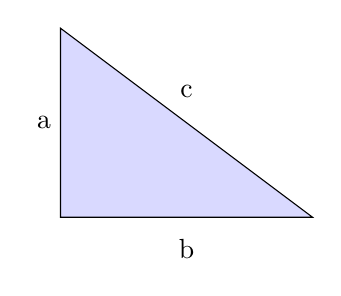
\begin{tikzpicture}[scale=.8]
	
		\path[draw, fill=blue!15 ] (0,0)-- 
			(0,3) node[pos=.5,left] {a} -- 
			(4,0) --cycle;
			
			\node (c) at (2,2) {c};
			\node (b) at (2,-.5) {b};
			
	
	\end{tikzpicture}
\end{center}

\begin{enumerate}
	\item $a=10$, \hspace{1in} $b=\sqrt{21}$,\hspace{1in} $c=$\underline{\hspace{1in}}\\
	
	\item $a=$\underline{\hspace{1in}}, \hspace{.5cm} $b=80$,\hspace{1in} $c=82$\\
	
	\item $a=30$, \hspace{1in}$b=40$, \hspace{1in}$c=$\underline{\hspace{1in}}\\
	
	\item $a=1$, \hspace{1in}$b=$\underline{\hspace{1in}},\hspace{.5cm} $c=\sqrt{3}$\\
	
	\item $a=7$,\hspace{1in} $b=7$,\hspace{1in} $c=$\underline{\hspace{1in}}
\end{enumerate}


\hrulefill

\subsection*{The Distance Formula}

$$d=\sqrt{(x_{1}-x_{2})^{2}+(y_{1}-y_{2})^{2}}$$

Find the distance between the two points. (3 points each)\\

\begin{enumerate}[resume]
\begin{multicols}{2}
	
	\item $(5,-2),(-3,10)$\\
	
	\item $(-8,2),(-2,-4)$\\
	
	\item $(-10,-20),(-1,20)$\\
	
	\item $(-5,-10), (5,14)$\\


\end{multicols}
\end{enumerate}

\pagebreak

\subsection*{Equation of a Circle}

$$r^2=x^2+y^2$$

$$r^2=(x-h)^2+(y-k)^2$$

Write the equation of a circle with the following criteria. (2 points each)\\

\begin{enumerate}[resume]

	\item $r=5$, center at the origin\\
	
	\item $r=6$, center at $(-4,-7)$\\
	
	\item $r=3$, center at $(8,1)$\\
	
	\item $r=\sqrt{10}$, center at $(11,12)$\\
	
	\item $r=\sqrt{13}$, center at $(-14,0)$\\
	
	\item center at $(0,0)$, passes through the point $(55,48)$\\
	
	
\end{enumerate}

\hrulefill

Sketch the following equations. (3 points each)\\

\begin{enumerate}[resume]
\begin{multicols}{2}

	\item $x^2+y^2=25$\\
	
%	\includegraphics[scale=.75]{graph1.jpg}
	
	\item $(x-1)^2+(y+1)^2=16$\\
	
%	\includegraphics[scale=.75]{graph1.jpg}

\end{multicols}
\end{enumerate}

\section*{Answer Key}

\begin{multicols}{3}

Quiz 1
\begin{enumerate}

\item 26

\item 18

\item $\sqrt{2}$

\item $\sqrt{2}$

\item 5

\item 41

\item 13

\item $4\sqrt{13}$

\item $4^2=x^2+y^2$

\item $6^2=(x+3)^2+(x+4)^2$

\item $2^2=x^2+(y-7)^2$

\item $3=(x-9)^2+(y-7)^2$

\item $7=(x-6)^2+y^2$

\item $65^2=x^2+y^2$\\


\end{enumerate}

Quiz 2

\begin{enumerate}

\item 13

\item 9

\item 15

\item $\sqrt{5}$

\item $2\sqrt{2}$

\item 41

\item $4\sqrt{13}$

\item 5

\item 13

\item $1=x^2+y^2$

\item $2^2=(x-3)^2+(Y+4)^2$

\item $3^2=(x+2)^2+(y-12)^2$

\item $5=(x+10)^2+(y+10)^2$

\item $11=(x+1)^2+(y-2)^2$

\item $65=(x+10)^2+(y+10)^2$

\end{enumerate}

quiz 3

\begin{enumerate}

\item $3\sqrt{2}$

\item 74

\item $\sqrt{5}$

\item 25

\item 39

\item 13

\item 5

\item 41

\item $4\sqrt{13}$

\item $10^2=x^2+y^2$

\item $9^2=(x+8)^2+(y+7)^2$

\item $6^2=(x-5)^2+(y+4)^2$

\item  $3=(x-2)^2+(x-1)^2$

\item $8=(x+4)^2+y^2$

\item $61^2=X^2+y^2$

\end{enumerate}
\end{multicols}

\hrulefill


Quiz 4

\begin{multicols}{2}
\begin{enumerate}

\item 11

\item 18

\item 50

\item $\sqrt{2}$

\item $7\sqrt{2}$

\item $4\sqrt{13}$

\item $6\sqrt{2}$

\item 41

\item 26

\item $5^2=x^2+y^2$

\item $6^2=(x+4)^2+(y+7)^2$

\item $3^2=(x-8)^2+(y-1)^2$

\item $10=(x-11)^2+(y-12)^2$

\item $13=(x+14)^2+y^2$

\item $73^2=x^2+y^2$

\end{enumerate}
\end{multicols}

\end{document}